% !TeX program = xelatex
\documentclass[10pt]{beamer}

\usetheme{metropolis}

\usepackage{pgfplots}
\usepgfplotslibrary{fillbetween}
\usepackage{pgfopts}
\usepackage{amsmath}
\usepackage{structuralanalysis}
\usepackage{tikz}
\usepackage{tikz-3dplot}
\usepackage{chngcntr}
\usepackage{wasysym}
\usepackage{mathtools}
\usepackage{alphalph}
\usepackage{xcolor}
\usepackage[showdow=false, en-US]{datetime2}
\usepackage{hyperref}

\newcommand{\highlight}[1]{%
	\colorbox{red!50}{$\displaystyle#1$}}

\setcounter{lecture}{19}
\counterwithin{equation}{lecture}
\makeatletter
\def\user@resume{resume}
\def\user@intermezzo{intermezzo}
%
\newcounter{previousequation}
\newcounter{lastsubequation}
\newcounter{savedparentequation}
\setcounter{savedparentequation}{1}
% 
\renewenvironment{subequations}[1][]{%
	\def\user@decides{#1}%
	\setcounter{previousequation}{\value{equation}}%
	\ifx\user@decides\user@resume 
	\setcounter{equation}{\value{savedparentequation}}%
	\else  
	\ifx\user@decides\user@intermezzo
	\refstepcounter{equation}%
	\else
	\setcounter{lastsubequation}{0}%
	\refstepcounter{equation}%
	\fi\fi
	\protected@edef\theHparentequation{%
		\@ifundefined {theHequation}\theequation \theHequation}%
	\protected@edef\theparentequation{\theequation}%
	\setcounter{parentequation}{\value{equation}}%
	\ifx\user@decides\user@resume 
	\setcounter{equation}{\value{lastsubequation}}%
	\else
	\setcounter{equation}{0}%
	\fi
	\def\theequation  {\theparentequation  \alph{equation}}%
	\def\theHequation {\theHparentequation \alph{equation}}%
	\ignorespaces
}{%
%  \arabic{equation};\arabic{savedparentequation};\arabic{lastsubequation}
\ifx\user@decides\user@resume
\setcounter{lastsubequation}{\value{equation}}%
\setcounter{equation}{\value{previousequation}}%
\else
\ifx\user@decides\user@intermezzo
\setcounter{equation}{\value{parentequation}}%
\else
\setcounter{lastsubequation}{\value{equation}}%
\setcounter{savedparentequation}{\value{parentequation}}%
\setcounter{equation}{\value{parentequation}}%
\fi\fi
%  \arabic{equation};\arabic{savedparentequation};\arabic{lastsubequation}
\ignorespacesafterend
}
\makeatother
\title{AE 737 - Mechanics of Damage Tolerance}
\subtitle{Lecture \arabic{lecture}}
\date{Last Updated: \today\ at \DTMcurrenttime}
\author{Dr. Nicholas Smith}
\institute{Wichita State University, Department of Aerospace Engineering}
% \titlegraphic{\hfill\includegraphics[height=1.5cm]{logo/logo}}

\begin{document}

\maketitle
\begin{frame}{schedule}
	\begin{itemize}
		\item 5 Apr - Crack Growth, Homework 7 due, Homework 8 assigned
		\item 7 Apr - Crack Growth, Stress Spectrum
		\item 12 Apr - Retardation, Boeing Commercial Method
		\item 14 Apr - Exam Review, Homework 8 Due
		\item 19 Apr - Exam 2
		\item 21 Apr - Exam Solutions, Damage Tolerance
%		\item 26 Apr - Damage Tolerance, AFGROW
%		\item 28 Apr - AFGROW, Finite Elements
%		\item 3 May - Finite Elements
%		\item 5 May - Non-Destructive Testing, Composites, Final Project Due May 10
	\end{itemize}
\end{frame}

\begin{frame}{final project clarification}
	\begin{itemize}[<+->]
		\item Some of the wording I used in the final project description is ambiguous, and based on what I learned in my fatigue class (not your text)
		\item By "crack growth" I intended "crack nucleation," which is a phrase to describe stress and strain based fatigue analysis
		\item "Crack propagation" is what I intended by what your text calls "crack growth", and refers to fracture mechanics-based fatigue analysis
	\end{itemize}
\end{frame}

\begin{frame}{office hours}
	\begin{itemize}
		\item I have a meeting this Friday afternoon (4/8)
		\item Office hours will be Monday 4/11 from 3:00 - 5:00
		\item As always you can e-mail me to schedule another time, or ask your questions via e-mail
	\end{itemize}
\end{frame}

\begin{frame}
  \frametitle{outline}
  \setbeamertemplate{section in toc}[sections numbered]
  \tableofcontents[hideallsubsections]
\end{frame}

\section{mean stress effects}
%mean stress
\begin{frame}{mean stress in strain-based fatigue}
	\begin{itemize}[<+->]
		\item In regions where plastic strain is significant, some applied mean stress is likely to be relaxed through cyclic plastic strain
		\item When the plastic strain is not significant, mean stress will exist
		\item Mean strain does not generally affect fatigue life
	\end{itemize}
\end{frame}

\begin{frame}{morrow approach}
	\begin{itemize}[<+->]
		\item Recall the Morrow approach for mean stress effects from the stress-based method
		\item[]\begin{equation}
		\frac{\sigma_a}{\sigma_{ar}} + \frac{\sigma_m}{\sigma_f^\prime} = 1
		\end{equation}
		\item We can rearrange the equation such that
		\item[]\begin{equation}
		\sigma_a = \sigma_f^\prime\left[\left(1-\frac{\sigma_m}{\sigma_f^\prime}\right)^\frac{1}{b}(2N_f)\right]^b
		\end{equation}
	\end{itemize}
\end{frame}

\begin{frame}{morrow approach}
	\begin{itemize}[<+->]
		\item If we compare to the stress-life equation ($\sigma_a = \sigma_f^\prime(2N_f)^b$), we see that we can replace $N_f$ with
		\item[] \begin{equation}
		\label{eq:nstar}
		N^* = N_f \left(1-\frac{\sigma_m}{\sigma_f^\prime}\right)^\frac{1}{b}
		\end{equation}
		\item We can now substitute $N^*$ for $N_f$ in the strain-life equation to find
		\item[] \begin{equation}
		\epsilon_a = \frac{\sigma_f^\prime}{E} \left(1-\frac{\sigma_m}{\sigma_f^\prime}\right)(2N_f)^b + \epsilon_f^\prime\left(1-\frac{\sigma_m}{\sigma_f^\prime}\right)^\frac{c}{b} (2 N_f)^c
		\end{equation}
	\end{itemize}
\end{frame}

\begin{frame}{morrow approach}
	\begin{itemize}[<+->]
		\item Graphically, we can use the Morrow approach very easily using only the zero-mean stress graph
		\item From the zero-mean stress graph, find the point corresponding to your applied strain
		\item For a non zero mean stress, this point represents $(\epsilon_a, N^*)$, we can now solve for $N_f$ using \ref{eq:nstar}
	\end{itemize}
\end{frame}

\begin{frame}{modified morrow}
	\begin{itemize}[<+->]
		\item While the Morrow equation agrees very well with many data, some are better fit with a modification
		\item In the modified version, it is assumed that the mean stress has no effect on the plastic term
		\item[] \begin{equation}
		\epsilon_a = \frac{\sigma_f^\prime}{E}\left(1-\frac{\sigma_f}{\sigma_f^\prime}\right)(2N_f)^b + \epsilon_f^\prime (2N_f)^c
		\end{equation}
		\item There is no convenient solution method for this form, and it generally must be solved numerically, or plotted with many families of $\sigma_m$
	\end{itemize}
\end{frame}

\begin{frame}{smith watson topper}
	\begin{itemize}[<+->]
		\item The Smith, Watson, and Topper approach assumes that the life for any given state is dependent on the product $\sigma_max \epsilon_a$
		\item After some manipulation, this gives
		\item[] \begin{equation}
		\sigma_{max} \epsilon_a = \frac{\left(\sigma_f^\prime\right)^2}{E}(2N_f)^{2b} + \sigma_f^\prime \epsilon_f^\prime (2N_f)^{b+c}
		\end{equation}
		\item This method can also be solved graphically if a plot of $\sigma_{max} \epsilon_a$ is made using zero-mean data. All we need to do is find the new $\sigma_{max} \epsilon_a$ point to find a new $N_f$
	\end{itemize}
\end{frame}

\begin{frame}{comparison}
	\begin{itemize}[<+->]
		\item All three methods discussed are in general use
		\item The Morrow method is very good for steel
		\item The modified Morrow method gives improved results in many materials
		\item The SWT approach is very good for general use, but is non-conservative with a compressive mean stress
	\end{itemize}
\end{frame}

\begin{frame}{example}
	
\end{frame}

\section{multiaxial loading}
%multiaxial loading

\begin{frame}{multiaxial loading}
	\begin{itemize}[<+->]
		\item Multi-axial loading in strain-based fatigue analysis is still an active field of research
		\item We are currently only capable of handling proportional loads that are in-phase (i.e. have the same frequency)
		\item If we consider the principal directions where $\sigma_{2a} = \lambda \sigma_{1a}$, we find an expression for the strain-life as
		\item[] \begin{equation}
		\epsilon_{1a} = \frac{\frac{\sigma_f^\prime}{E}(1-\nu \lambda)(2N_f)^b + \epsilon_f^\prime(1-0.5\lambda)(2N_f)^c}{\sqrt{1-\lambda+\lambda^2}}
		\end{equation}
	\end{itemize}
\end{frame}

\begin{frame}{stress triaxiality factor}
	\begin{itemize}[<+->]
		\item Another approach is to consider the stress triaxiality factor
		\item[] \begin{equation}
		T = \frac{1+\lambda}{\sqrt{1-\lambda+\lambda^2}}
		\end{equation}
		\item Three notable cases of this are
		\begin{enumerate}
			\item Pure planar shear: $\lambda=-1, T=0$
			\item Uniaxial stress: $\lambda=0, T=1$
			\item Equal biaxial stress: $\lambda=1, T=2$
		\end{enumerate}
		\item Marloff suggests the following inclusion of stress triaxiality
		\item[] \begin{equation}
		\bar{\epsilon_a} = \frac{\sigma_f^\prime}{E}(2 N_f)^b + 2^{1-T}\epsilon_f^\prime(2N_f)^c
		\end{equation}
	\end{itemize}
\end{frame}

\section{crack growth rate}

\begin{frame}{fracture surface}
	\begin{figure}
	\centering
	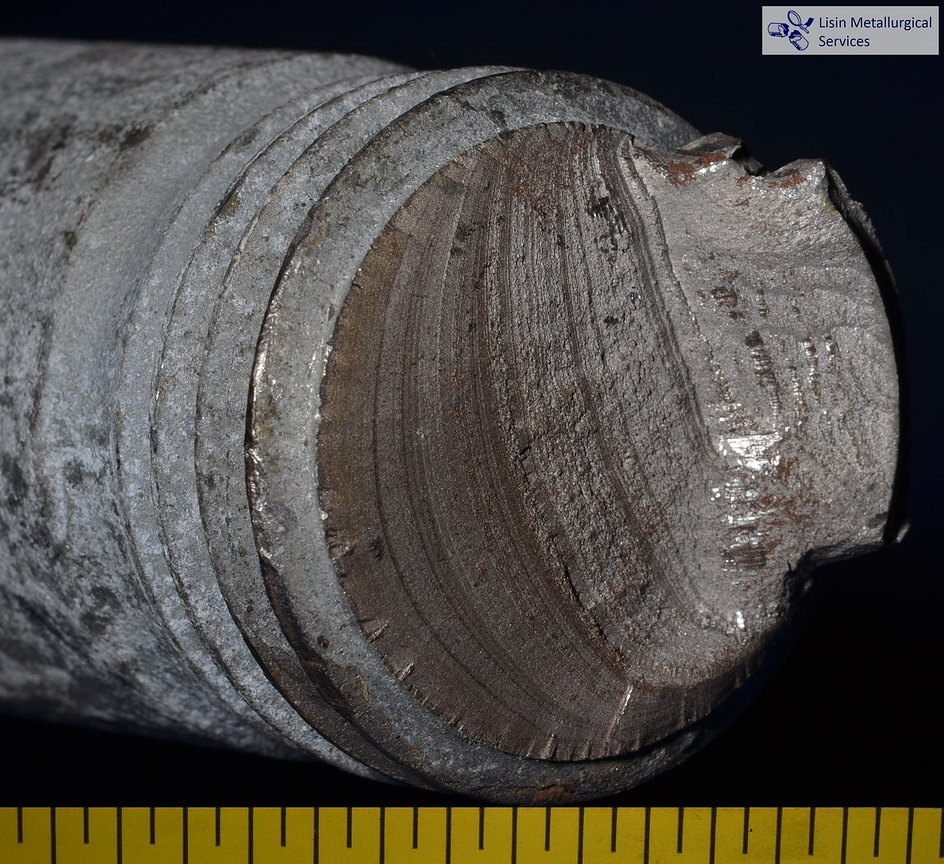
\includegraphics[width=0.7\linewidth]{../Figures/fracture_surface}
	\label{fig:fracture_surface}
	\end{figure}
\end{frame}

\begin{frame}{fracture surface}	
	\begin{figure}
	\centering
	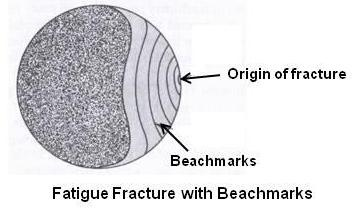
\includegraphics[width=0.7\linewidth]{../Figures/Fatigue-Fracture-with-Beachmarks}
	\label{fig:Fatigue-Fracture-with-Beachmarks}
	\end{figure}
\end{frame}

\begin{frame}{crack growth rate}
	\begin{itemize}[<+->]
	\item We can observe that fatigue damage occurs through crack propagation
	\item "cracks" and fracture mechanics have been omitted from all our fatigue discussion thus far
	\item It would be beneficial to predict at what rate a crack will extend
	\end{itemize}
\end{frame}

\begin{frame}{crack growth rate}
	\begin{itemize}[<+->]
		\item Crack growth rate can be measured experimentally 
		\item Using a center-crack specimen, a fatigue load is applied
		\item The crack length is measured and plotted vs. the number of cycles
		\item The slope of this curve ($\frac{da}{dN}$) is then plotted vs. either $K_{I,max}$ or $\Delta K_I$ on a log-log scale
		\item This chart is then commonly divided into three regions
	\end{itemize}
\end{frame}

\begin{frame}{da-dN vs K}	
	\begin{figure}
	\centering
	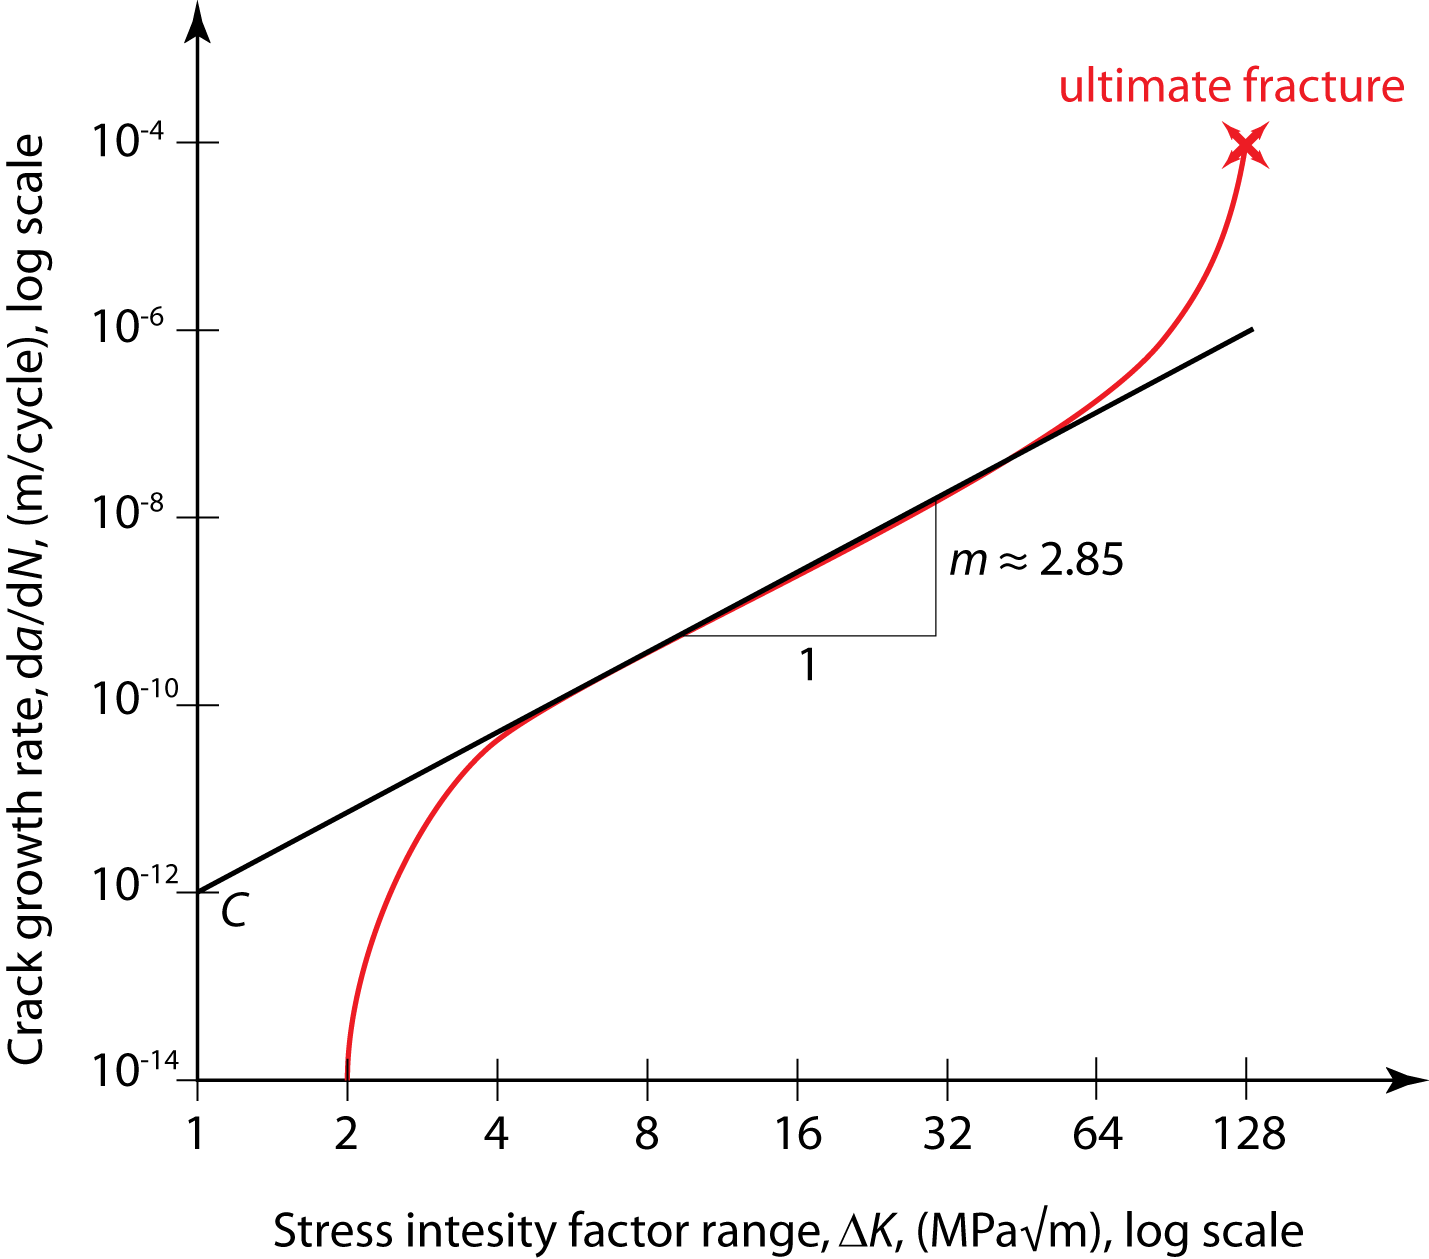
\includegraphics[width=0.7\linewidth]{../Figures/da-dn}
	\label{fig:da-dn}
	\end{figure}
\end{frame}

\begin{frame}{region I}
	\begin{itemize}[<+->]
		\item In Region I crack growth is very slow and/or difficult to measure
		\item In many cases, da/dN corresponds to the spacing between atoms!
		\item The point at which the da/dN curve intersects the boundary between Region I and Region II is often called the fatigue threshold
		\item Typically 3-15 $\text{ ksi} \sqrt{\text{in}}$ for steel
		\item 3-6 $\text{ ksi} \sqrt{\text{in}}$ for aluminum
	\end{itemize}
\end{frame}

\begin{frame}{region II}
	\begin{itemize}[<+->]
		\item Most important region for general engineering analysis
		\item Once a crack is present, most of the growth and life occurs in Region II
		\item Generally linear in the log-log scale
	\end{itemize}
\end{frame}

\begin{frame}{region III}
	\begin{itemize}[<+->]
		\item Unstable crack growth
		\item Usually neglected (we expect failure before Region III fully develops in actual parts)
		\item Can be significant for parts where we expect high stress and relatively short life
	\end{itemize}
\end{frame}

\begin{frame}{crack growth rate curve}
	\begin{itemize}[<+->]
		\item The crack growth rate curve is considered a material property
		\item The same considerations for thickness apply as with fracture toughness ($K_c$ vs. $K_{Ic}$) 
		\item Is also a function of the load ratio, $R = \sigma_{min}/\sigma_{max}$
	\end{itemize}
\end{frame}

\begin{frame}{R effects}
	\begin{itemize}[<+->]
		\item While the x-axis can be either $\Delta K$ or $K_{max}$, the shape of the data is the same
		\item When we look at the effects of load ratio, $R$, the axis causes some differences on the plot
		\item With $\Delta K$ on the x-axis, increasing $R$ will shift the curve up and to the left, shifting the fatigue threshold and fracture toughness on the graph as well
		\item With $K_{max}$ on the x-axis, increasing $R$ shifts the curve down and to the right, but fatigue threshold and fracture toughness keep same values
		\item In general, $R$ dependence vanishes for $R> 0.8$ or $R<-0.3$. This effect is known as the band width
	\end{itemize}
\end{frame}

\section{crack growth rate equations}

%TODO plots/sketches of growth rate equations
\begin{frame}{crack growth rate equations}
	\begin{itemize}[<+->]
		\item There are many crack growth rate equations of varying complexity
		\item The "best" form to use will depend on design needs\
		\item The important features in curve-fit equations are
		\begin{enumerate}
			\item Region II curve fit (linear on log-log scale)
			\item Region I curve fit (fatigue threshold)
			\item Region III curve fit (critical stress intensity)
			\item Stress ratio effects
			\item Band width of R-curves
		\end{enumerate}
	\end{itemize}
\end{frame}

\begin{frame}{paris law}
	\begin{itemize}[<+->]
		\item The original
		\item Fits the linear portion (Region II)
		\item Does not fit Region I, Region III, or have R-dependence
		\item[]\begin{equation}
		\frac{da}{dN} = C (\Delta K)^n
		\end{equation}
		\item Note: this assumes the x-axis is $\Delta K$, but $\Delta K = (1-R) K_{max}$, so we can easily convert
	\end{itemize}
\end{frame}

\begin{frame}{paris law}
	\begin{tikzpicture}
	\begin{axis}[
	xmode=log,
	ymode=log
	]
	\addplot [mark=none]{10^(-10)*x^4};
	\end{axis}
	\end{tikzpicture}
\end{frame}

\begin{frame}{walker}
	\begin{itemize}[<+->]
		\item Region II is usually all that is needed for engineering, but R-dependence is often an important effect to capture
		\item Walker modified the Paris law to account for R-dependence
		\item[] \begin{equation}
		\frac{da}{dN} = C\left[(1-R)^mK_{max}\right]^n
		\end{equation}
		\item Gives a good fit for Region II with R-dependence and band width
	\end{itemize}
\end{frame}

\begin{frame}{walker}
	\begin{tikzpicture}
	\begin{axis}[
	xmode=log,
	ymode=log
	]
	\addplot [mark=none]{10^(-10)*x^4};
	\addplot [mark=none]{10^(-10)*((1-0.33)^(.2)*x)^4};
	\addplot [mark=none]{10^(-10)*((1-0.5)^(.2)*x)^4};
	\addplot [mark=none]{10^(-10)*((1-0.7)^(.2)*x)^4};
	\end{axis}
	\end{tikzpicture}
\end{frame}

\begin{frame}{forman}
	\begin{itemize}[<+->]
		\item The Forman equation was developed to capture the effects of Region II and Region III
		\item Also includes the effects of $R$, but does not control the band width of R effects
		\item[] \begin{equation}
		\frac{da}{dN} = \frac{C \left[(1-R)K_{max}\right]^n}{(1-R)K_c-(1-R)K_{max}}
		\end{equation}
	\end{itemize}
\end{frame}

\begin{frame}{modified forman}
	\begin{itemize}[<+->]
		\item The Forman equation can be modified to include the effect of band width
		\item[] \begin{equation}
		\frac{da}{dN} = \frac{C \left[(1-R)^m K_{max}\right]^n}{\left[(1-R)^mK_c-(1-R)^m K_{max}\right]^L}
		\end{equation}
	\end{itemize}
\end{frame}

\begin{frame}{collipriest}
	\begin{itemize}[<+->]
		\item The Collipriest equation fits Regions I, II and III, but has no R-dependence
		\item[] \begin{equation}
		\frac{da}{dN} = C_1 + C_2 \tanh^{-1} \left[\frac{\log \left(\frac{K_{max}^2}{K_oK_c}\right)}{\log (K_c/K_o)}\right]
		\end{equation}
	\end{itemize}
\end{frame}

\begin{frame}{modified collipriest}
	\begin{itemize}[<+->]
		\item Following the same methods as before, we can modify the Collipriest equation for R-dependence and band width control
		\item [] \begin{equation}
		\frac{da}{dN} = C_1 + C_2 \tanh^{-1} \left[\frac{\log \left(\frac{(1-R)^mK_{max}^2}{K_oK_c}\right)}{\log (K_c/K_o)}\right]
		\end{equation}
		\item For a cleaner graph, experimental data at different R-values is sometimes plotted vs. $K_{eff}$
		\item[] \begin{equation}
		K_{eff} = (1-R)^m K_{max}
		\end{equation}
	\end{itemize}
\end{frame}

\begin{frame}{nasgrow growth rate equation}
	\begin{itemize}[<+->]
		\item A very complicated curve fit is provided in the NASGROW growth rate equation
		\item[] \begin{equation}
		\frac{da}{dN} = C \left[\frac{1-f}{1-R}\Delta K\right]^n\frac{\left[1-\frac{\Delta K_{th}}{\Delta K}\right]}{\left[1-\frac{K_{max}}{K_{crit}}\right]}
		\end{equation}
		\item The curve fit parameters can be found in p. 307 of your text (or the NASGROLW/AFGROW documentation)
	\end{itemize}
\end{frame}

\begin{frame}{boeing-walker growth rate equation}
	\begin{itemize}[<+->]
		\item The Boeing-Walker growth equation is given as (for $R \ge 0$ )
		\item[] \begin{equation}
		\frac{da}{dN} = 10^{-4}\left(\frac{1}{mT}\right)^p\left[K_max(1-R)^q\right]^p
		\end{equation}
	\end{itemize}
\end{frame}

\begin{frame}{conversion of constants}
	\begin{itemize}[<+->]
		\item Much of the data available to us is from Boeing, and given in terms of the Boeing-Walker equation
		\item We can re-write some other equations to more easily convert parameters between the various equations
		\item Walker-Boeing:
		\begin{equation}
		\frac{da}{dN} = 10^{-4}\left(\frac{1}{mT}\right)^p\left[\Delta K(1-R)^{q-1}\right]^p
		\end{equation}
		\item Walker-AFGROW:
		\begin{equation}
		\frac{da}{dN} = C_w\left[\Delta K(1-R)^{m-1}\right]^{n_w}
		\end{equation}
		\item Forman:
		\begin{equation}
		\frac{da}{dN} = \frac{C_F}{(1-R)K_c - \Delta K} (\Delta K)^{n_f}
		\end{equation}
	\end{itemize}
\end{frame}

\begin{frame}{conversion of constants}
	\begin{tabular}{ccc}
	Walker-Boeing	& Walker-AFGROW & Forman \\ 
	\hline
	$10^{-4}\left(\frac{1}{mT}\right)^p$	& $C_w = 10^{-4}\left(\frac{1}{mT}\right)^p$ & $C_F = (K_c-1)10^{-4}\left(\frac{1}{mT}\right)^p$ \\ 
	q	& $m=q$ &  \\ 
	p	& $n_w = p$ & $n_f = p$ \\ 
	\end{tabular} 
\end{frame}
\end{document}
